\section{Planificación}

El proyecto se desarrolló en tres fases: preproducción, desarrollo y postproducción. Cada fase contiene una serie de tareas a realizar, con una estimación en horas para cada fase \tabref{tab:fases_tareas}.

\begin{table}[H]
    \caption{Fases, estimación y tareas.}\label{tab:fases_tareas}
    \scriptsize
    \centering
    \begin{tabular}{lllp{0.45\textwidth}}
        \hline

        \textbf{Fase} & \textbf{Estimación} & \textbf{Tarea} & \textbf{Descripción} \\ \hline
        
        \multirow{2}{*}{Preproducción} 
        & 12h & 1.1 & Investigación de estado del arte. \\ 
        & 4h & 1.2 & Selección de tecnologías y herramientas. \\ \hline
        
        \multirow{6}{*}{Desarrollo} 
        & 50h & 2.1 & Configuración del proyecto, implementación de estructura básica de la web, autenticación y perfil de usuario. \\ 
        & 50h & 2.2 & Desarrollo de algoritmo de cálculo de acordes. \\ 
        & 50h & 2.3 & Implementación de páginas para la visualización y creación de publicaciones. \\ 
        & 36h & 2.4 & Desarrollo de biblioteca de publicaciones. \\ 
        & 24h & 2.5 & Implementación de componentes sociales. \\ 
        & 24h & 2.6 & Desarrollo de páginas informativas. \\ \hline
        
        \multirow{2}{*}{Postproducción} 
        & 46h & 3.1 & Redacción de memoria. \\ 
        & 4h & 3.2 & Elaboración de presentación. \\ \hline
        
    \end{tabular}
\end{table}

Además, durante la fase de \textbf{desarrollo} se aplicó la \textbf{metodología iterativa e icremental}, siendo cada tarea equivalente a un incremento \tabref{tab:incrementos}.

\begin{table}[H]
    \centering
    \scriptsize
    \caption{Fase de desarrollo; incrementos y descripción.}\label{tab:incrementos}
    \begin{tabular}{cp{0.6\textwidth}}
        \hline
        \textbf{Incremento} & \textbf{Descripción} \\ \hline
        1 & Configuración del proyecto, implementación de estructura básica de la web, autenticación y perfil de usuario. \\ 
        2 & Desarrollo de algoritmo de cálculo de acordes. \\
        3 & Implementación de páginas para la visualización y creación de publicaciones. \\
        4 & Desarrollo de biblioteca de publicaciones. \\
        5 & Implementación de componentes sociales. \\ 
        6 & Desarrollo de páginas informativas. \\ \hline
    \end{tabular}
\end{table}

Finalmente, durante la ejecución de cada incremento se siguió una variación del flujo de desarrollo mencionado anteriormente, sustituyendo al entrega por el despliegue del incremento, y añadiendo las fases de preproducción y postproducción como actividades de inicio y final respectivamente. \figref{fig:flujo_met}.

\begin{figure}[H]
    \centering
    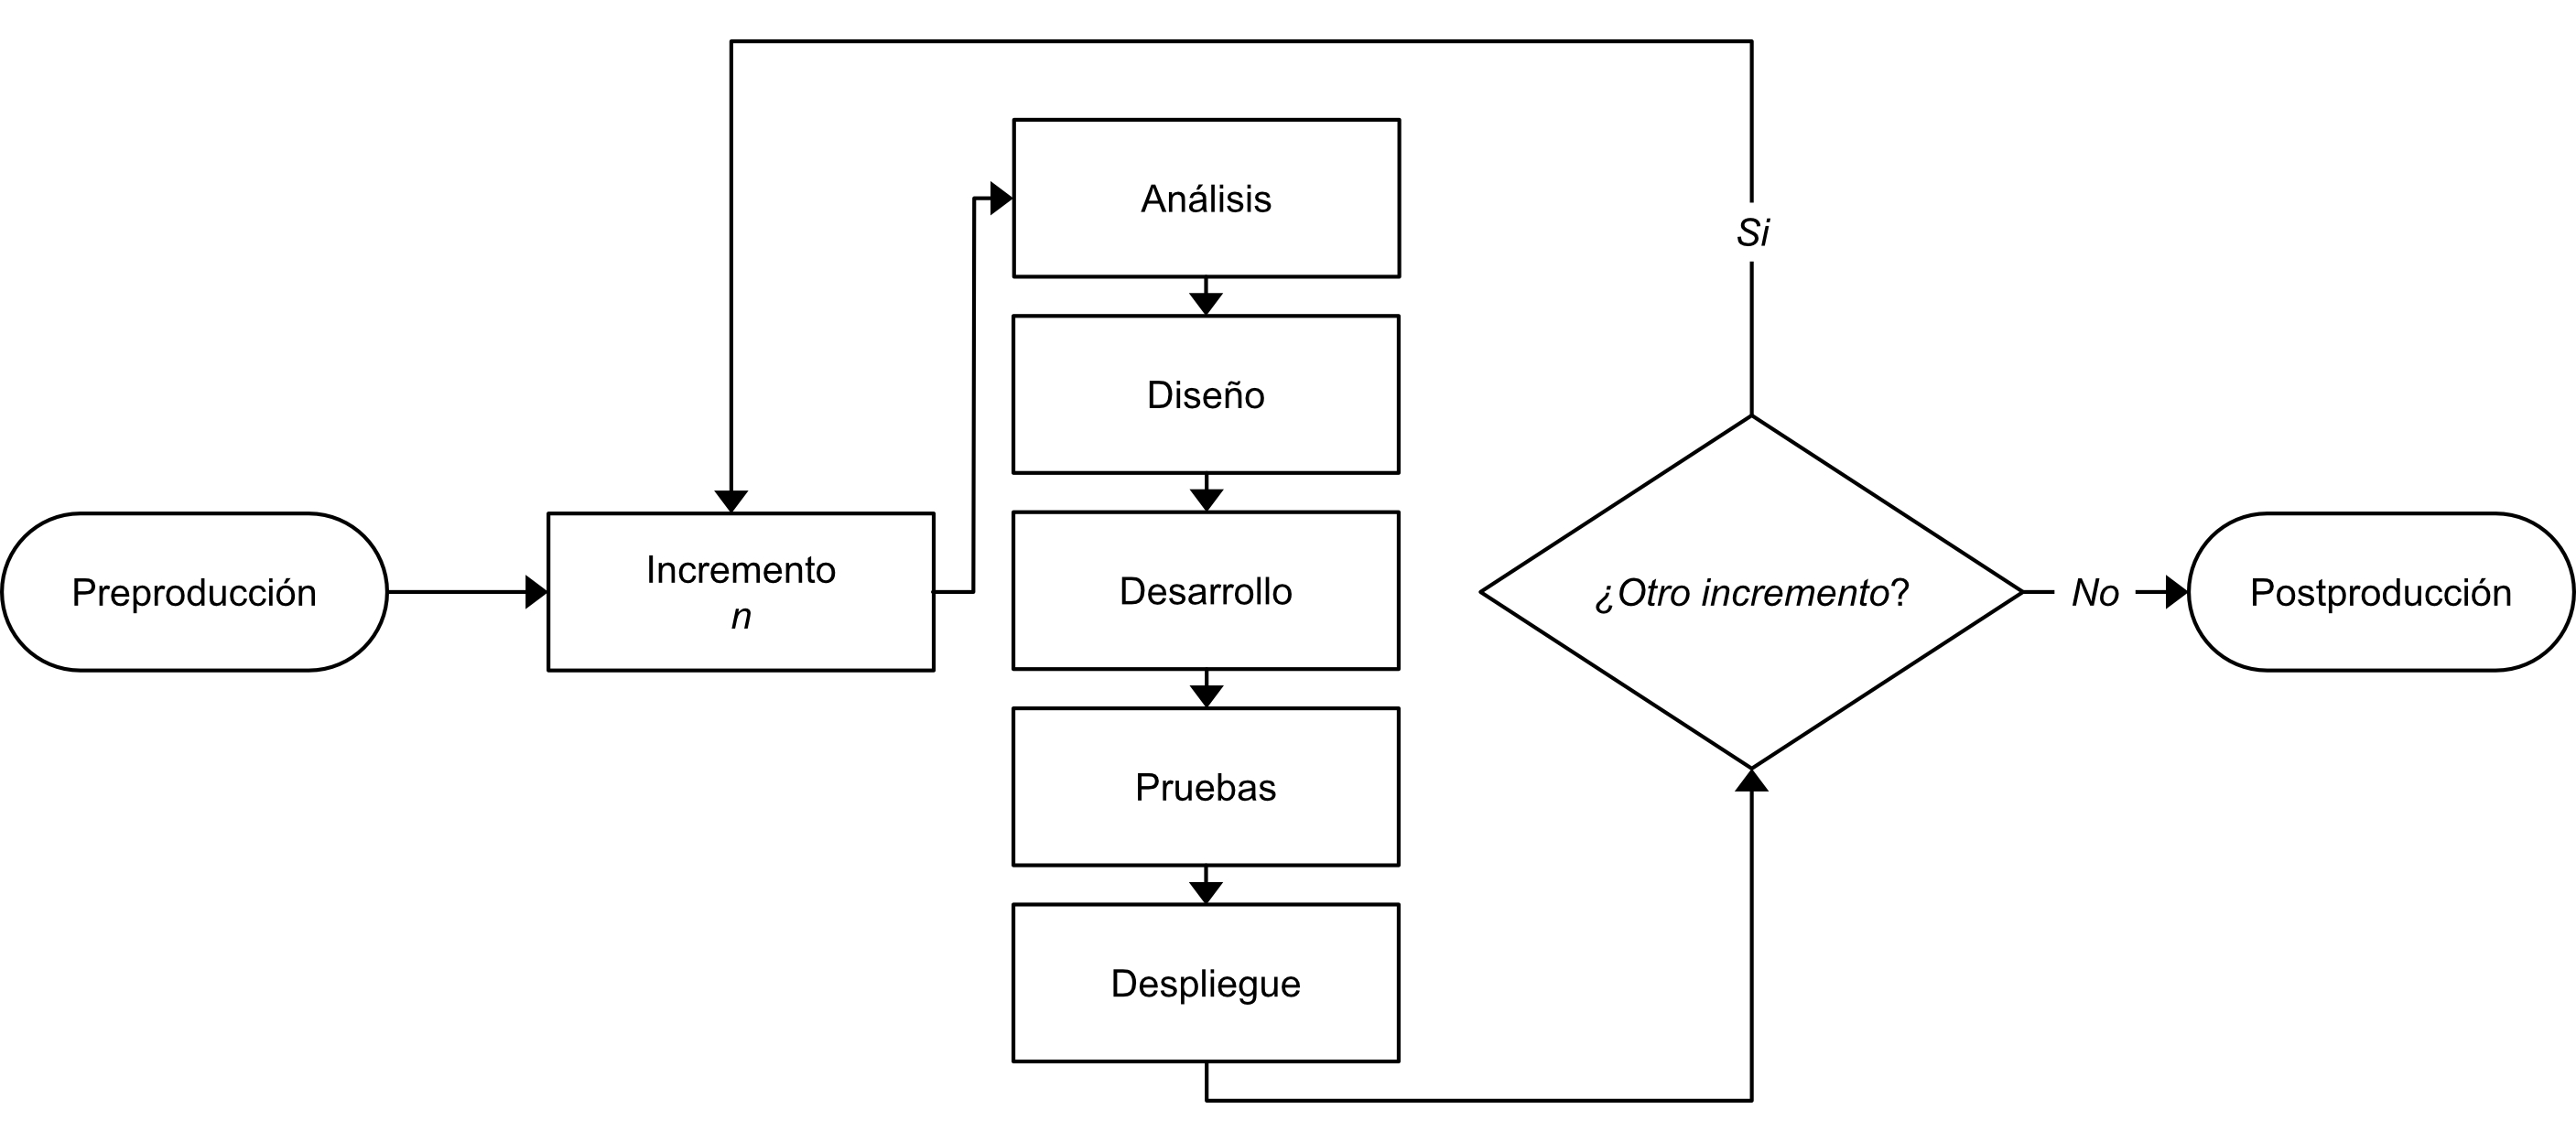
\includegraphics[width=1\textwidth]{Ilustraciones/metodologia/flujo_met.jpg}
    \caption{Proceso de desarrollo adaptado al proyecto}
    \label{fig:flujo_met}
\end{figure}